\documentclass[1p]{elsarticle_modified}
%\bibliographystyle{elsarticle-num}

%\usepackage[colorlinks]{hyperref}
%\usepackage{abbrmath_seonhwa} %\Abb, \Ascr, \Acal ,\Abf, \Afrak
\usepackage{amsfonts}
\usepackage{amssymb}
\usepackage{amsmath}
\usepackage{amsthm}
\usepackage{scalefnt}
\usepackage{amsbsy}
\usepackage{kotex}
\usepackage{caption}
\usepackage{subfig}
\usepackage{color}
\usepackage{graphicx}
\usepackage{xcolor} %% white, black, red, green, blue, cyan, magenta, yellow
\usepackage{float}
\usepackage{setspace}
\usepackage{hyperref}

\usepackage{tikz}
\usetikzlibrary{arrows}

\usepackage{multirow}
\usepackage{array} % fixed length table
\usepackage{hhline}

%%%%%%%%%%%%%%%%%%%%%
\makeatletter
\renewcommand*\env@matrix[1][\arraystretch]{%
	\edef\arraystretch{#1}%
	\hskip -\arraycolsep
	\let\@ifnextchar\new@ifnextchar
	\array{*\c@MaxMatrixCols c}}
\makeatother %https://tex.stackexchange.com/questions/14071/how-can-i-increase-the-line-spacing-in-a-matrix
%%%%%%%%%%%%%%%

\usepackage[normalem]{ulem}

\newcommand{\msout}[1]{\ifmmode\text{\sout{\ensuremath{#1}}}\else\sout{#1}\fi}
%SOURCE: \msout is \stkout macro in https://tex.stackexchange.com/questions/20609/strikeout-in-math-mode

\newcommand{\cancel}[1]{
	\ifmmode
	{\color{red}\msout{#1}}
	\else
	{\color{red}\sout{#1}}
	\fi
}

\newcommand{\add}[1]{
	{\color{blue}\uwave{#1}}
}

\newcommand{\replace}[2]{
	\ifmmode
	{\color{red}\msout{#1}}{\color{blue}\uwave{#2}}
	\else
	{\color{red}\sout{#1}}{\color{blue}\uwave{#2}}
	\fi
}

\newcommand{\Sol}{\mathcal{S}} %segment
\newcommand{\D}{D} %diagram
\newcommand{\A}{\mathcal{A}} %arc


%%%%%%%%%%%%%%%%%%%%%%%%%%%%%5 test

\def\sl{\operatorname{\textup{SL}}(2,\Cbb)}
\def\psl{\operatorname{\textup{PSL}}(2,\Cbb)}
\def\quan{\mkern 1mu \triangleright \mkern 1mu}

\theoremstyle{definition}
\newtheorem{thm}{Theorem}[section]
\newtheorem{prop}[thm]{Proposition}
\newtheorem{lem}[thm]{Lemma}
\newtheorem{ques}[thm]{Question}
\newtheorem{cor}[thm]{Corollary}
\newtheorem{defn}[thm]{Definition}
\newtheorem{exam}[thm]{Example}
\newtheorem{rmk}[thm]{Remark}
\newtheorem{alg}[thm]{Algorithm}

\newcommand{\I}{\sqrt{-1}}
\begin{document}

%\begin{frontmatter}
%
%\title{Boundary parabolic representations of knots up to 8 crossings}
%
%%% Group authors per affiliation:
%\author{Yunhi Cho} 
%\address{Department of Mathematics, University of Seoul, Seoul, Korea}
%\ead{yhcho@uos.ac.kr}
%
%
%\author{Seonhwa Kim} %\fnref{s_kim}}
%\address{Center for Geometry and Physics, Institute for Basic Science, Pohang, 37673, Korea}
%\ead{ryeona17@ibs.re.kr}
%
%\author{Hyuk Kim}
%\address{Department of Mathematical Sciences, Seoul National University, Seoul 08826, Korea}
%\ead{hyukkim@snu.ac.kr}
%
%\author{Seokbeom Yoon}
%\address{Department of Mathematical Sciences, Seoul National University, Seoul, 08826,  Korea}
%\ead{sbyoon15@snu.ac.kr}
%
%\begin{abstract}
%We find all boundary parabolic representation of knots up to 8 crossings.
%
%\end{abstract}
%\begin{keyword}
%    \MSC[2010] 57M25 
%\end{keyword}
%
%\end{frontmatter}

%\linenumbers
%\tableofcontents
%
\newcommand\colored[1]{\textcolor{white}{\rule[-0.35ex]{0.8em}{1.4ex}}\kern-0.8em\color{red} #1}%
%\newcommand\colored[1]{\textcolor{white}{ #1}\kern-2.17ex	\textcolor{white}{ #1}\kern-1.81ex	\textcolor{white}{ #1}\kern-2.15ex\color{red}#1	}

{\Large $\underline{12a_{0348}~(K12a_{0348})}$}

\setlength{\tabcolsep}{10pt}
\renewcommand{\arraystretch}{1.6}
\vspace{1cm}\begin{tabular}{m{100pt}>{\centering\arraybackslash}m{274pt}}
\multirow{5}{120pt}{
	\centering
	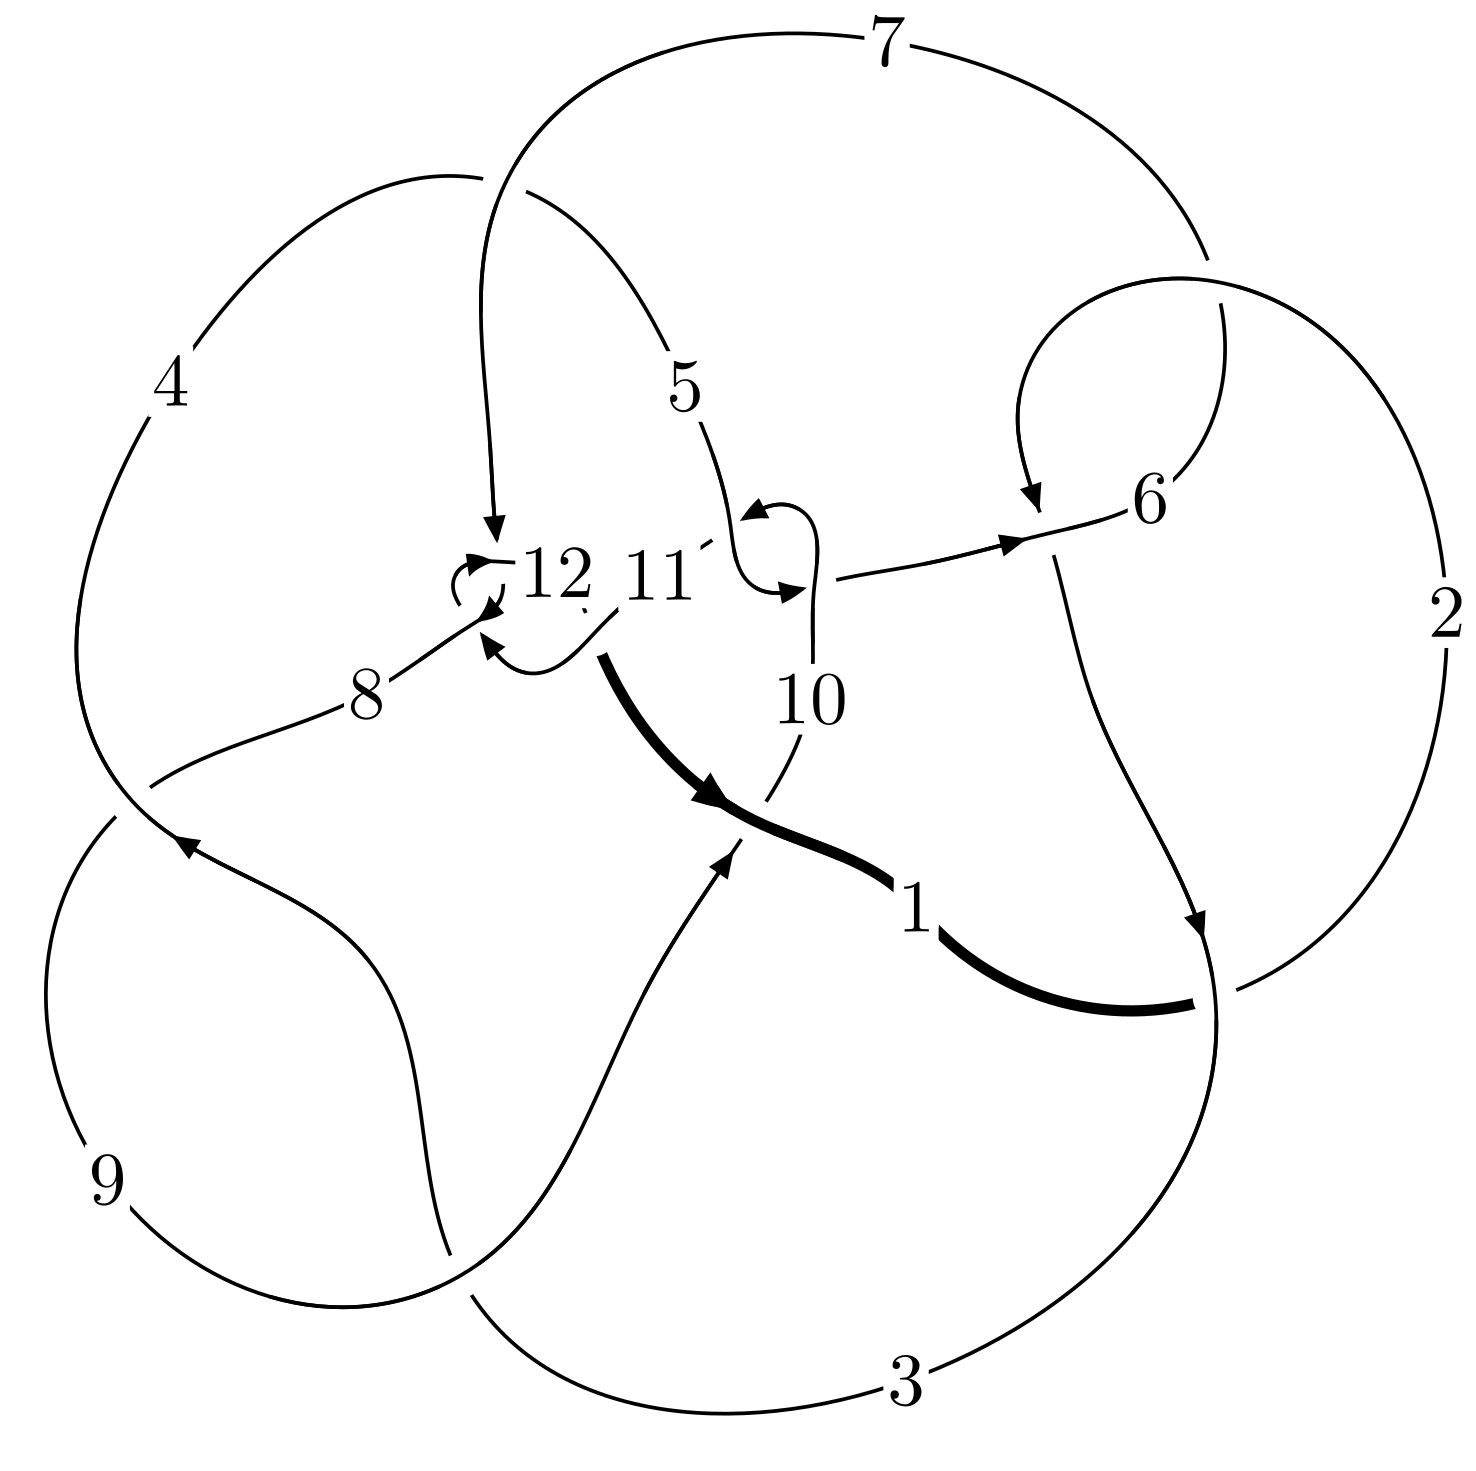
\includegraphics[width=112pt]{../../../GIT/diagram.site/diagram/png/1149_12a_0348.png}\\
\ \ \ A knot diagram\footnotemark}&
\allowdisplaybreaks
\textbf{Linearized knot diagam} \\
\cline{2-2}
 &
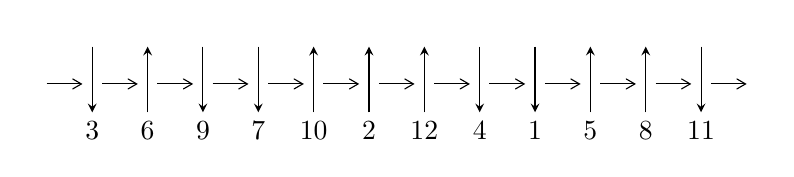
\begin{tikzpicture}[x=20pt, y=17pt]
	% nodes
	\node (C0) at (0, 0) {};
	\node (C1) at (1, 0) {};
	\node (C1U) at (1, +1) {};
	\node (C1D) at (1, -1) {3};

	\node (C2) at (2, 0) {};
	\node (C2U) at (2, +1) {};
	\node (C2D) at (2, -1) {6};

	\node (C3) at (3, 0) {};
	\node (C3U) at (3, +1) {};
	\node (C3D) at (3, -1) {9};

	\node (C4) at (4, 0) {};
	\node (C4U) at (4, +1) {};
	\node (C4D) at (4, -1) {7};

	\node (C5) at (5, 0) {};
	\node (C5U) at (5, +1) {};
	\node (C5D) at (5, -1) {10};

	\node (C6) at (6, 0) {};
	\node (C6U) at (6, +1) {};
	\node (C6D) at (6, -1) {2};

	\node (C7) at (7, 0) {};
	\node (C7U) at (7, +1) {};
	\node (C7D) at (7, -1) {12};

	\node (C8) at (8, 0) {};
	\node (C8U) at (8, +1) {};
	\node (C8D) at (8, -1) {4};

	\node (C9) at (9, 0) {};
	\node (C9U) at (9, +1) {};
	\node (C9D) at (9, -1) {1};

	\node (C10) at (10, 0) {};
	\node (C10U) at (10, +1) {};
	\node (C10D) at (10, -1) {5};

	\node (C11) at (11, 0) {};
	\node (C11U) at (11, +1) {};
	\node (C11D) at (11, -1) {8};

	\node (C12) at (12, 0) {};
	\node (C12U) at (12, +1) {};
	\node (C12D) at (12, -1) {11};
	\node (C13) at (13, 0) {};

	% arrows
	\draw[->,>={angle 60}]
	(C0) edge (C1) (C1) edge (C2) (C2) edge (C3) (C3) edge (C4) (C4) edge (C5) (C5) edge (C6) (C6) edge (C7) (C7) edge (C8) (C8) edge (C9) (C9) edge (C10) (C10) edge (C11) (C11) edge (C12) (C12) edge (C13) ;	\draw[->,>=stealth]
	(C1U) edge (C1D) (C2D) edge (C2U) (C3U) edge (C3D) (C4U) edge (C4D) (C5D) edge (C5U) (C6D) edge (C6U) (C7D) edge (C7U) (C8U) edge (C8D) (C9U) edge (C9D) (C10D) edge (C10U) (C11D) edge (C11U) (C12U) edge (C12D) ;
	\end{tikzpicture} \\
\hhline{~~} \\& 
\textbf{Solving Sequence} \\ \cline{2-2} 
 &
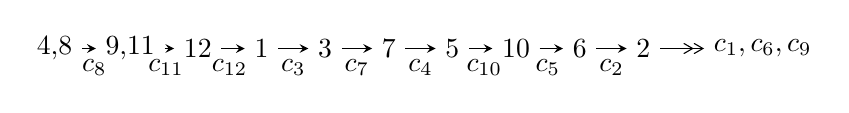
\begin{tikzpicture}[x=23pt, y=7pt]
	% node
	\node (A0) at (-1/8, 0) {4,8};
	\node (A1) at (17/16, 0) {9,11};
	\node (A2) at (17/8, 0) {12};
	\node (A3) at (25/8, 0) {1};
	\node (A4) at (33/8, 0) {3};
	\node (A5) at (41/8, 0) {7};
	\node (A6) at (49/8, 0) {5};
	\node (A7) at (57/8, 0) {10};
	\node (A8) at (65/8, 0) {6};
	\node (A9) at (73/8, 0) {2};
	\node (C1) at (1/2, -1) {$c_{8}$};
	\node (C2) at (13/8, -1) {$c_{11}$};
	\node (C3) at (21/8, -1) {$c_{12}$};
	\node (C4) at (29/8, -1) {$c_{3}$};
	\node (C5) at (37/8, -1) {$c_{7}$};
	\node (C6) at (45/8, -1) {$c_{4}$};
	\node (C7) at (53/8, -1) {$c_{10}$};
	\node (C8) at (61/8, -1) {$c_{5}$};
	\node (C9) at (69/8, -1) {$c_{2}$};
	\node (A10) at (11, 0) {$c_{1},c_{6},c_{9}$};

	% edge
	\draw[->,>=stealth]	
	(A0) edge (A1) (A1) edge (A2) (A2) edge (A3) (A3) edge (A4) (A4) edge (A5) (A5) edge (A6) (A6) edge (A7) (A7) edge (A8) (A8) edge (A9) ;
	\draw[->>,>={angle 60}]	
	(A9) edge (A10);
\end{tikzpicture} \\ 

\end{tabular} \\

\footnotetext{
The image of knot diagram is generated by the software ``\textbf{Draw programme}" developed by Andrew Bartholomew(\url{http://www.layer8.co.uk/maths/draw/index.htm\#Running-draw}), where we modified some parts for our purpose(\url{https://github.com/CATsTAILs/LinksPainter}).
}\phantom \\ \newline 
\centering \textbf{Ideals for irreducible components\footnotemark of $X_{\text{par}}$} 
 
\begin{align*}
I^u_{1}&=\langle 
2.44733\times10^{21} u^{19}-1.13296\times10^{22} u^{18}+\cdots+5.42213\times10^{21} b-2.42529\times10^{22},\\
\phantom{I^u_{1}}&\phantom{= \langle  }-1.95629\times10^{21} u^{19}+5.54886\times10^{22} u^{18}+\cdots+2.41285\times10^{23} a+6.92349\times10^{23},\\
\phantom{I^u_{1}}&\phantom{= \langle  }9 u^{20}-45 u^{19}+\cdots-430 u+89\rangle \\
I^u_{2}&=\langle 
-2.31722\times10^{21} u^{33}-5.93285\times10^{21} u^{32}+\cdots-2.13415\times10^{21} a+2.34088\times10^{21},\\
\phantom{I^u_{2}}&\phantom{= \langle  }8.20059\times10^{21} a u^{33}+9.19800\times10^{21} u^{33}+\cdots-7.14710\times10^{21} a-3.57339\times10^{22},\;3 u^{34}+6 u^{33}+\cdots+u^2+1\rangle \\
I^u_{3}&=\langle 
b,\;a-1,\;u^4- u^3+2 u^2-2 u+1\rangle \\
I^u_{4}&=\langle 
- u^3+b- u+1,\;- u^3+u^2+a-2 u,\;u^4- u^3+2 u^2-2 u+1\rangle \\
I^u_{5}&=\langle 
b,\;a-1,\;u^2+u+1\rangle \\
I^u_{6}&=\langle 
b- u,\;a,\;u^2+u+1\rangle \\
I^u_{7}&=\langle 
- a u+b+a+u-1,\;2 a^2- a u-3 a+2 u+1,\;u^2+1\rangle \\
I^u_{8}&=\langle 
b^2+b+1,\;- u^5 a^2+2 u^5 a+\cdots-2 b-1,\;- u^3 a+u^3+b u- a u+b+u,\\
\phantom{I^u_{8}}&\phantom{= \langle  }u^6 a^2-2 u^6 a+2 u^4 a^2+u^6-3 u^4 a+a^2 u^2+u^3 a+u^4- u^2 a- u^3+a u+u^2+u+1\rangle \\
I^u_{9}&=\langle 
- u^5 a^2+2 u^5 a-2 u^3 a^2- u^5+3 u^3 a- a^2 u+u^2 a- u^3+a u- u^2+b+a- u,\\
\phantom{I^u_{9}}&\phantom{= \langle  }u^6 a^2-2 u^6 a+2 u^4 a^2+u^6-3 u^4 a+a^2 u^2-2 u^3 a+u^4- u^2 a+2 u^3-2 a u+u^2+u+1\rangle \\
\\
\end{align*}
\raggedright * 7 irreducible components of $\dim_{\mathbb{C}}=0$, with total 104 representations.\\
\raggedright * 2 irreducible components of $\dim_{\mathbb{C}}=1$ \\
\footnotetext{All coefficients of polynomials are rational numbers. But the coefficients are sometimes approximated in decimal forms when there is not enough margin.}
\newpage
\renewcommand{\arraystretch}{1}
\centering \section*{I. $I^u_{1}= \langle 2.45\times10^{21} u^{19}-1.13\times10^{22} u^{18}+\cdots+5.42\times10^{21} b-2.43\times10^{22},\;-1.96\times10^{21} u^{19}+5.55\times10^{22} u^{18}+\cdots+2.41\times10^{23} a+6.92\times10^{23},\;9 u^{20}-45 u^{19}+\cdots-430 u+89 \rangle$}
\flushleft \textbf{(i) Arc colorings}\\
\begin{tabular}{m{7pt} m{180pt} m{7pt} m{180pt} }
\flushright $a_{4}=$&$\begin{pmatrix}0\\u\end{pmatrix}$ \\
\flushright $a_{8}=$&$\begin{pmatrix}1\\0\end{pmatrix}$ \\
\flushright $a_{9}=$&$\begin{pmatrix}1\\u^2\end{pmatrix}$ \\
\flushright $a_{11}=$&$\begin{pmatrix}0.00810779 u^{19}-0.229972 u^{18}+\cdots+10.0312 u-2.86943\\-0.451360 u^{19}+2.08951 u^{18}+\cdots-19.3998 u+4.47296\end{pmatrix}$ \\
\flushright $a_{12}=$&$\begin{pmatrix}-0.443253 u^{19}+1.85954 u^{18}+\cdots-9.36858 u+1.60353\\-0.451360 u^{19}+2.08951 u^{18}+\cdots-19.3998 u+4.47296\end{pmatrix}$ \\
\flushright $a_{1}=$&$\begin{pmatrix}-0.211003 u^{19}+0.993904 u^{18}+\cdots-3.69980 u+1.00079\\0.0403786 u^{19}-0.205972 u^{18}+\cdots+0.306071 u-0.245024\end{pmatrix}$ \\
\flushright $a_{3}=$&$\begin{pmatrix}u\\u^3+u\end{pmatrix}$ \\
\flushright $a_{7}=$&$\begin{pmatrix}0.0858884 u^{19}-0.602361 u^{18}+\cdots+12.6293 u-2.96434\\-0.149037 u^{19}+0.448835 u^{18}+\cdots-0.0305593 u-0.376609\end{pmatrix}$ \\
\flushright $a_{5}=$&$\begin{pmatrix}0.225218 u^{19}-1.17037 u^{18}+\cdots+15.3833 u-4.17263\\-0.277055 u^{19}+0.981406 u^{18}+\cdots+0.712270 u-0.967405\end{pmatrix}$ \\
\flushright $a_{10}=$&$\begin{pmatrix}0.142110 u^{19}-0.738313 u^{18}+\cdots+10.1501 u-1.73455\\-0.0701601 u^{19}+0.526991 u^{18}+\cdots-9.31954 u+2.50170\end{pmatrix}$ \\
\flushright $a_{6}=$&$\begin{pmatrix}0.262889 u^{19}-1.03833 u^{18}+\cdots+8.32215 u-2.29128\\-0.0555259 u^{19}+0.0487443 u^{18}+\cdots+8.11030 u-2.81062\end{pmatrix}$ \\
\flushright $a_{2}=$&$\begin{pmatrix}0.0853475 u^{19}-0.306104 u^{18}+\cdots+3.79747 u-0.473020\\0.251374 u^{19}-1.26858 u^{18}+\cdots+13.5561 u-3.51608\end{pmatrix}$\\&\end{tabular}
\flushleft \textbf{(ii) Obstruction class $= -1$}\\~\\
\flushleft \textbf{(iii) Cusp Shapes $= -\frac{18263454827549106375}{169441495364258615324} u^{19}-\frac{59899476849528023793}{42360373841064653831} u^{18}+\cdots+\frac{14114427005478277957347}{169441495364258615324} u-\frac{4369480590430740839387}{169441495364258615324}$}\\~\\
\newpage\renewcommand{\arraystretch}{1}
\flushleft \textbf{(iv) u-Polynomials at the component}\newline \\
\begin{tabular}{m{50pt}|m{274pt}}
Crossings & \hspace{64pt}u-Polynomials at each crossing \\
\hline $$\begin{aligned}c_{1},c_{12}\end{aligned}$$&$\begin{aligned}
&u^{20}+12 u^{19}+\cdots+27 u+4
\end{aligned}$\\
\hline $$\begin{aligned}c_{2},c_{6},c_{7}\\c_{11}\end{aligned}$$&$\begin{aligned}
&u^{20}+2 u^{19}+\cdots+u+2
\end{aligned}$\\
\hline $$\begin{aligned}c_{3},c_{8}\end{aligned}$$&$\begin{aligned}
&9(9 u^{20}+45 u^{19}+\cdots+430 u+89)
\end{aligned}$\\
\hline $$\begin{aligned}c_{4},c_{9}\end{aligned}$$&$\begin{aligned}
&4(4 u^{20}-8 u^{19}+\cdots+33 u^2+9)
\end{aligned}$\\
\hline $$\begin{aligned}c_{5},c_{10}\end{aligned}$$&$\begin{aligned}
&9(9 u^{20}+45 u^{19}+\cdots+268 u+89)
\end{aligned}$\\
\hline
\end{tabular}\\~\\
\newpage\renewcommand{\arraystretch}{1}
\flushleft \textbf{(v) Riley Polynomials at the component}\newline \\
\begin{tabular}{m{50pt}|m{274pt}}
Crossings & \hspace{64pt}Riley Polynomials at each crossing \\
\hline $$\begin{aligned}c_{1},c_{12}\end{aligned}$$&$\begin{aligned}
&y^{20}-8 y^{19}+\cdots+655 y+16
\end{aligned}$\\
\hline $$\begin{aligned}c_{2},c_{6},c_{7}\\c_{11}\end{aligned}$$&$\begin{aligned}
&y^{20}+12 y^{19}+\cdots+27 y+4
\end{aligned}$\\
\hline $$\begin{aligned}c_{3},c_{8}\end{aligned}$$&$\begin{aligned}
&81(81 y^{20}+1161 y^{19}+\cdots+40982 y+7921)
\end{aligned}$\\
\hline $$\begin{aligned}c_{4},c_{9}\end{aligned}$$&$\begin{aligned}
&16(16 y^{20}+80 y^{19}+\cdots+594 y+81)
\end{aligned}$\\
\hline $$\begin{aligned}c_{5},c_{10}\end{aligned}$$&$\begin{aligned}
&81(81 y^{20}+837 y^{19}+\cdots+66838 y+7921)
\end{aligned}$\\
\hline
\end{tabular}\\~\\
\newpage\flushleft \textbf{(vi) Complex Volumes and Cusp Shapes}
$$\begin{array}{c|c|c}  
\text{Solutions to }I^u_{1}& \I (\text{vol} + \sqrt{-1}CS) & \text{Cusp shape}\\
 \hline 
\begin{aligned}
u &= \phantom{-}0.092200 + 1.047180 I \\
a &= \phantom{-}0.004677 + 0.790560 I \\
b &= -0.09546 - 1.64917 I\end{aligned}
 & -8.80426 - 0.45536 I & \phantom{-}1.9853 + 17.0975 I \\ \hline\begin{aligned}
u &= \phantom{-}0.092200 - 1.047180 I \\
a &= \phantom{-}0.004677 - 0.790560 I \\
b &= -0.09546 + 1.64917 I\end{aligned}
 & -8.80426 + 0.45536 I & \phantom{-}1.9853 - 17.0975 I \\ \hline\begin{aligned}
u &= \phantom{-}0.848738 + 0.341219 I \\
a &= -0.396390 + 0.042942 I \\
b &= \phantom{-}0.693866 + 0.427483 I\end{aligned}
 & \phantom{-}0.08901 - 2.93076 I & \phantom{-}1.95121 + 2.50627 I \\ \hline\begin{aligned}
u &= \phantom{-}0.848738 - 0.341219 I \\
a &= -0.396390 - 0.042942 I \\
b &= \phantom{-}0.693866 - 0.427483 I\end{aligned}
 & \phantom{-}0.08901 + 2.93076 I & \phantom{-}1.95121 - 2.50627 I \\ \hline\begin{aligned}
u &= \phantom{-}0.613570 + 0.532135 I \\
a &= -1.169550 - 0.185382 I \\
b &= \phantom{-}0.168318 - 1.217040 I\end{aligned}
 & -9.43070 - 2.05540 I & -10.55085 + 3.27009 I \\ \hline\begin{aligned}
u &= \phantom{-}0.613570 - 0.532135 I \\
a &= -1.169550 + 0.185382 I \\
b &= \phantom{-}0.168318 + 1.217040 I\end{aligned}
 & -9.43070 + 2.05540 I & -10.55085 - 3.27009 I \\ \hline\begin{aligned}
u &= -0.479857 + 0.602074 I \\
a &= \phantom{-}0.353859 - 1.186080 I \\
b &= \phantom{-}0.026282 - 0.889205 I\end{aligned}
 & -2.87875 + 1.45206 I & -8.03079 - 4.11530 I \\ \hline\begin{aligned}
u &= -0.479857 - 0.602074 I \\
a &= \phantom{-}0.353859 + 1.186080 I \\
b &= \phantom{-}0.026282 + 0.889205 I\end{aligned}
 & -2.87875 - 1.45206 I & -8.03079 + 4.11530 I \\ \hline\begin{aligned}
u &= \phantom{-}1.256360 + 0.179722 I \\
a &= -0.906871 - 0.475961 I \\
b &= \phantom{-}0.603304 - 1.077240 I\end{aligned}
 & -3.61567 - 12.98850 I & -3.22409 + 10.41992 I \\ \hline\begin{aligned}
u &= \phantom{-}1.256360 - 0.179722 I \\
a &= -0.906871 + 0.475961 I \\
b &= \phantom{-}0.603304 + 1.077240 I\end{aligned}
 & -3.61567 + 12.98850 I & -3.22409 - 10.41992 I\\
 \hline 
 \end{array}$$\newpage$$\begin{array}{c|c|c}  
\text{Solutions to }I^u_{1}& \I (\text{vol} + \sqrt{-1}CS) & \text{Cusp shape}\\
 \hline 
\begin{aligned}
u &= \phantom{-}0.202083 + 0.692929 I \\
a &= \phantom{-}0.668174 + 0.227261 I \\
b &= -0.254612 + 0.364368 I\end{aligned}
 & \phantom{-}0.359490 - 1.106510 I & \phantom{-}4.17160 + 6.47143 I \\ \hline\begin{aligned}
u &= \phantom{-}0.202083 - 0.692929 I \\
a &= \phantom{-}0.668174 - 0.227261 I \\
b &= -0.254612 - 0.364368 I\end{aligned}
 & \phantom{-}0.359490 + 1.106510 I & \phantom{-}4.17160 - 6.47143 I \\ \hline\begin{aligned}
u &= \phantom{-}0.37431 + 1.41465 I \\
a &= \phantom{-}1.021310 + 0.740873 I \\
b &= -0.944071 - 0.466625 I\end{aligned}
 & \phantom{-}5.54214 - 7.36961 I & \phantom{-}4.38642 + 3.37286 I \\ \hline\begin{aligned}
u &= \phantom{-}0.37431 - 1.41465 I \\
a &= \phantom{-}1.021310 - 0.740873 I \\
b &= -0.944071 + 0.466625 I\end{aligned}
 & \phantom{-}5.54214 + 7.36961 I & \phantom{-}4.38642 - 3.37286 I \\ \hline\begin{aligned}
u &= -0.33594 + 1.49255 I \\
a &= -1.032280 + 0.658846 I \\
b &= \phantom{-}0.816010 - 0.603612 I\end{aligned}
 & \phantom{-}8.32420 + 1.49101 I & \phantom{-}7.14130 + 1.02494 I \\ \hline\begin{aligned}
u &= -0.33594 - 1.49255 I \\
a &= -1.032280 - 0.658846 I \\
b &= \phantom{-}0.816010 + 0.603612 I\end{aligned}
 & \phantom{-}8.32420 - 1.49101 I & \phantom{-}7.14130 - 1.02494 I \\ \hline\begin{aligned}
u &= \phantom{-}0.54073 + 1.45381 I \\
a &= \phantom{-}1.82309 + 0.12465 I \\
b &= -0.682856 + 1.134390 I\end{aligned}
 & \phantom{-}1.4774 - 19.2240 I & -0.44918 + 10.82584 I \\ \hline\begin{aligned}
u &= \phantom{-}0.54073 - 1.45381 I \\
a &= \phantom{-}1.82309 - 0.12465 I \\
b &= -0.682856 - 1.134390 I\end{aligned}
 & \phantom{-}1.4774 + 19.2240 I & -0.44918 - 10.82584 I \\ \hline\begin{aligned}
u &= -0.61219 + 1.52578 I \\
a &= -1.62445 + 0.10961 I \\
b &= \phantom{-}0.669219 + 1.040740 I\end{aligned}
 & \phantom{-}5.64729 + 12.61550 I & \phantom{-}2.61904 - 9.47385 I \\ \hline\begin{aligned}
u &= -0.61219 - 1.52578 I \\
a &= -1.62445 - 0.10961 I \\
b &= \phantom{-}0.669219 - 1.040740 I\end{aligned}
 & \phantom{-}5.64729 - 12.61550 I & \phantom{-}2.61904 + 9.47385 I\\
 \hline 
 \end{array}$$\newpage\newpage\renewcommand{\arraystretch}{1}
\centering \section*{II. $I^u_{2}= \langle -2.32\times10^{21} u^{33}-5.93\times10^{21} u^{32}+\cdots-2.13\times10^{21} a+2.34\times10^{21},\;8.20\times10^{21} a u^{33}+9.20\times10^{21} u^{33}+\cdots-7.15\times10^{21} a-3.57\times10^{22},\;3 u^{34}+6 u^{33}+\cdots+u^2+1 \rangle$}
\flushleft \textbf{(i) Arc colorings}\\
\begin{tabular}{m{7pt} m{180pt} m{7pt} m{180pt} }
\flushright $a_{4}=$&$\begin{pmatrix}0\\u\end{pmatrix}$ \\
\flushright $a_{8}=$&$\begin{pmatrix}1\\0\end{pmatrix}$ \\
\flushright $a_{9}=$&$\begin{pmatrix}1\\u^2\end{pmatrix}$ \\
\flushright $a_{11}=$&$\begin{pmatrix}a\\1.08578 u^{33}+2.77996 u^{32}+\cdots+a-1.09687\end{pmatrix}$ \\
\flushright $a_{12}=$&$\begin{pmatrix}1.08578 u^{33}+2.77996 u^{32}+\cdots+2 a-1.09687\\1.08578 u^{33}+2.77996 u^{32}+\cdots+a-1.09687\end{pmatrix}$ \\
\flushright $a_{1}=$&$\begin{pmatrix}1.97436 a u^{33}-16.8142 u^{33}+\cdots-3.43039 a+13.1329\\0.681005 a u^{33}-1.25817 u^{33}+\cdots-0.357162 a+0.186404\end{pmatrix}$ \\
\flushright $a_{3}=$&$\begin{pmatrix}u\\u^3+u\end{pmatrix}$ \\
\flushright $a_{7}=$&$\begin{pmatrix}-0.589433 a u^{33}-1.32608 u^{33}+\cdots+0.705146 a+13.5864\\0.514636 a u^{33}-1.30333 u^{33}+\cdots-0.245900 a+4.59327\end{pmatrix}$ \\
\flushright $a_{5}=$&$\begin{pmatrix}-7.17034 a u^{33}+27.2048 u^{33}+\cdots+5.86324 a-7.07975\\-2.39818 a u^{33}+3.29061 u^{33}+\cdots+0.291662 a+2.38603\end{pmatrix}$ \\
\flushright $a_{10}=$&$\begin{pmatrix}12.4359 u^{33}+3 a u^{32}+\cdots+a-33.6250\\-0.874985 a u^{33}+5.42874 u^{33}+\cdots+1.39011 a-9.26373\end{pmatrix}$ \\
\flushright $a_{6}=$&$\begin{pmatrix}-3 a u^{33}+1.73278 u^{33}+\cdots+42.6932 u+6.26647\\-0.608399 u^{33}-1.49941 u^{32}+\cdots+1.09687 u+0.361927\end{pmatrix}$ \\
\flushright $a_{2}=$&$\begin{pmatrix}1.04587 a u^{33}-17.2962 u^{33}+\cdots-3.60194 a+13.7910\\0.263401 a u^{33}-1.07806 u^{33}+\cdots-0.456131 a+0.659305\end{pmatrix}$\\&\end{tabular}
\flushleft \textbf{(ii) Obstruction class $= -1$}\\~\\
\flushleft \textbf{(iii) Cusp Shapes $= -\frac{110192114528878828278}{33346026295216206221} u^{33}-\frac{312161458732301950125}{133384105180864824884} u^{32}+\cdots-\frac{118687147920568685837}{66692052590432412442} u-\frac{611488195859711746311}{133384105180864824884}$}\\~\\
\newpage\renewcommand{\arraystretch}{1}
\flushleft \textbf{(iv) u-Polynomials at the component}\newline \\
\begin{tabular}{m{50pt}|m{274pt}}
Crossings & \hspace{64pt}u-Polynomials at each crossing \\
\hline $$\begin{aligned}c_{1},c_{12}\end{aligned}$$&$\begin{aligned}
&u^{68}+28 u^{67}+\cdots+3540540 u+405769
\end{aligned}$\\
\hline $$\begin{aligned}c_{2},c_{6},c_{7}\\c_{11}\end{aligned}$$&$\begin{aligned}
&u^{68}+4 u^{67}+\cdots+2840 u+637
\end{aligned}$\\
\hline $$\begin{aligned}c_{3},c_{8}\end{aligned}$$&$\begin{aligned}
&9(3 u^{34}-6 u^{33}+\cdots+u^2+1)^{2}
\end{aligned}$\\
\hline $$\begin{aligned}c_{4},c_{9}\end{aligned}$$&$\begin{aligned}
&64(64 u^{68}+64 u^{67}+\cdots+770022 u+2211093)
\end{aligned}$\\
\hline $$\begin{aligned}c_{5},c_{10}\end{aligned}$$&$\begin{aligned}
&9(3 u^{34}-6 u^{33}+\cdots-4 u+1)^{2}
\end{aligned}$\\
\hline
\end{tabular}\\~\\
\newpage\renewcommand{\arraystretch}{1}
\flushleft \textbf{(v) Riley Polynomials at the component}\newline \\
\begin{tabular}{m{50pt}|m{274pt}}
Crossings & \hspace{64pt}Riley Polynomials at each crossing \\
\hline $$\begin{aligned}c_{1},c_{12}\end{aligned}$$&$\begin{aligned}
&y^{68}+28 y^{67}+\cdots+3856761155056 y+164648481361
\end{aligned}$\\
\hline $$\begin{aligned}c_{2},c_{6},c_{7}\\c_{11}\end{aligned}$$&$\begin{aligned}
&y^{68}+28 y^{67}+\cdots+3540540 y+405769
\end{aligned}$\\
\hline $$\begin{aligned}c_{3},c_{8}\end{aligned}$$&$\begin{aligned}
&81(9 y^{34}+240 y^{33}+\cdots+2 y+1)^{2}
\end{aligned}$\\
\hline $$\begin{aligned}c_{4},c_{9}\end{aligned}$$&$\begin{aligned}
&4096\\
&\cdot(4096 y^{68}+106496 y^{67}+\cdots+7083972171144 y+4888932254649)
\end{aligned}$\\
\hline $$\begin{aligned}c_{5},c_{10}\end{aligned}$$&$\begin{aligned}
&81(9 y^{34}+168 y^{33}+\cdots+2 y+1)^{2}
\end{aligned}$\\
\hline
\end{tabular}\\~\\
\newpage\flushleft \textbf{(vi) Complex Volumes and Cusp Shapes}
$$\begin{array}{c|c|c}  
\text{Solutions to }I^u_{2}& \I (\text{vol} + \sqrt{-1}CS) & \text{Cusp shape}\\
 \hline 
\begin{aligned}
u &= \phantom{-}0.928923 + 0.129584 I \\
a &= -0.887196 - 0.818849 I \\
b &= \phantom{-}0.120625 - 1.127660 I\end{aligned}
 & -6.72431 + 5.79611 I & -7.79847 - 4.21340 I \\ \hline\begin{aligned}
u &= \phantom{-}0.928923 + 0.129584 I \\
a &= -0.487954 + 0.335298 I \\
b &= \phantom{-}0.579811 + 1.099130 I\end{aligned}
 & -6.72431 + 5.79611 I & -7.79847 - 4.21340 I \\ \hline\begin{aligned}
u &= \phantom{-}0.928923 - 0.129584 I \\
a &= -0.887196 + 0.818849 I \\
b &= \phantom{-}0.120625 + 1.127660 I\end{aligned}
 & -6.72431 - 5.79611 I & -7.79847 + 4.21340 I \\ \hline\begin{aligned}
u &= \phantom{-}0.928923 - 0.129584 I \\
a &= -0.487954 - 0.335298 I \\
b &= \phantom{-}0.579811 - 1.099130 I\end{aligned}
 & -6.72431 - 5.79611 I & -7.79847 + 4.21340 I \\ \hline\begin{aligned}
u &= -1.059230 + 0.243669 I \\
a &= -0.847568 + 0.653323 I \\
b &= \phantom{-}0.592845 + 1.069630 I\end{aligned}
 & -1.74401 + 7.89373 I & -0.77647 - 6.38566 I \\ \hline\begin{aligned}
u &= -1.059230 + 0.243669 I \\
a &= -0.610778 - 0.013981 I \\
b &= \phantom{-}0.736784 - 0.428981 I\end{aligned}
 & -1.74401 + 7.89373 I & -0.77647 - 6.38566 I \\ \hline\begin{aligned}
u &= -1.059230 - 0.243669 I \\
a &= -0.847568 - 0.653323 I \\
b &= \phantom{-}0.592845 - 1.069630 I\end{aligned}
 & -1.74401 - 7.89373 I & -0.77647 + 6.38566 I \\ \hline\begin{aligned}
u &= -1.059230 - 0.243669 I \\
a &= -0.610778 + 0.013981 I \\
b &= \phantom{-}0.736784 + 0.428981 I\end{aligned}
 & -1.74401 - 7.89373 I & -0.77647 + 6.38566 I \\ \hline\begin{aligned}
u &= \phantom{-}0.196215 + 1.099790 I \\
a &= \phantom{-}0.344789 + 0.498969 I \\
b &= -0.236178 + 1.094890 I\end{aligned}
 & \phantom{-}1.71677 - 1.07665 I & \phantom{-}3.45366 + 0.91009 I \\ \hline\begin{aligned}
u &= \phantom{-}0.196215 + 1.099790 I \\
a &= -1.19817 - 1.18268 I \\
b &= \phantom{-}0.753486 + 0.716576 I\end{aligned}
 & \phantom{-}1.71677 - 1.07665 I & \phantom{-}3.45366 + 0.91009 I\\
 \hline 
 \end{array}$$\newpage$$\begin{array}{c|c|c}  
\text{Solutions to }I^u_{2}& \I (\text{vol} + \sqrt{-1}CS) & \text{Cusp shape}\\
 \hline 
\begin{aligned}
u &= \phantom{-}0.196215 - 1.099790 I \\
a &= \phantom{-}0.344789 - 0.498969 I \\
b &= -0.236178 - 1.094890 I\end{aligned}
 & \phantom{-}1.71677 + 1.07665 I & \phantom{-}3.45366 - 0.91009 I \\ \hline\begin{aligned}
u &= \phantom{-}0.196215 - 1.099790 I \\
a &= -1.19817 + 1.18268 I \\
b &= \phantom{-}0.753486 - 0.716576 I\end{aligned}
 & \phantom{-}1.71677 + 1.07665 I & \phantom{-}3.45366 - 0.91009 I \\ \hline\begin{aligned}
u &= -0.411561 + 1.108320 I \\
a &= \phantom{-}0.173904 - 0.612229 I \\
b &= -0.143739 - 1.063970 I\end{aligned}
 & \phantom{-}0.82810 + 6.47536 I & \phantom{-}0.07862 - 6.80334 I \\ \hline\begin{aligned}
u &= -0.411561 + 1.108320 I \\
a &= -2.12606 + 0.12473 I \\
b &= \phantom{-}0.664230 + 0.990769 I\end{aligned}
 & \phantom{-}0.82810 + 6.47536 I & \phantom{-}0.07862 - 6.80334 I \\ \hline\begin{aligned}
u &= -0.411561 - 1.108320 I \\
a &= \phantom{-}0.173904 + 0.612229 I \\
b &= -0.143739 + 1.063970 I\end{aligned}
 & \phantom{-}0.82810 - 6.47536 I & \phantom{-}0.07862 + 6.80334 I \\ \hline\begin{aligned}
u &= -0.411561 - 1.108320 I \\
a &= -2.12606 - 0.12473 I \\
b &= \phantom{-}0.664230 - 0.990769 I\end{aligned}
 & \phantom{-}0.82810 - 6.47536 I & \phantom{-}0.07862 + 6.80334 I \\ \hline\begin{aligned}
u &= \phantom{-}0.061990 + 1.217400 I \\
a &= \phantom{-}1.271910 - 0.079555 I \\
b &= -0.594585 + 1.258760 I\end{aligned}
 & \phantom{-}2.60150 - 1.59411 I & \phantom{-}4.61171 + 4.12369 I \\ \hline\begin{aligned}
u &= \phantom{-}0.061990 + 1.217400 I \\
a &= -1.55260 - 0.58417 I \\
b &= \phantom{-}0.832284 + 1.073760 I\end{aligned}
 & \phantom{-}2.60150 - 1.59411 I & \phantom{-}4.61171 + 4.12369 I \\ \hline\begin{aligned}
u &= \phantom{-}0.061990 - 1.217400 I \\
a &= \phantom{-}1.271910 + 0.079555 I \\
b &= -0.594585 - 1.258760 I\end{aligned}
 & \phantom{-}2.60150 + 1.59411 I & \phantom{-}4.61171 - 4.12369 I \\ \hline\begin{aligned}
u &= \phantom{-}0.061990 - 1.217400 I \\
a &= -1.55260 + 0.58417 I \\
b &= \phantom{-}0.832284 - 1.073760 I\end{aligned}
 & \phantom{-}2.60150 + 1.59411 I & \phantom{-}4.61171 - 4.12369 I\\
 \hline 
 \end{array}$$\newpage$$\begin{array}{c|c|c}  
\text{Solutions to }I^u_{2}& \I (\text{vol} + \sqrt{-1}CS) & \text{Cusp shape}\\
 \hline 
\begin{aligned}
u &= -0.309763 + 1.205810 I \\
a &= \phantom{-}1.19397 - 0.75885 I \\
b &= -1.018550 + 0.481300 I\end{aligned}
 & -1.13644 + 4.47248 I & -0.55538 - 5.09131 I \\ \hline\begin{aligned}
u &= -0.309763 + 1.205810 I \\
a &= -0.267392 - 0.127975 I \\
b &= -0.024069 + 1.347120 I\end{aligned}
 & -1.13644 + 4.47248 I & -0.55538 - 5.09131 I \\ \hline\begin{aligned}
u &= -0.309763 - 1.205810 I \\
a &= \phantom{-}1.19397 + 0.75885 I \\
b &= -1.018550 - 0.481300 I\end{aligned}
 & -1.13644 - 4.47248 I & -0.55538 + 5.09131 I \\ \hline\begin{aligned}
u &= -0.309763 - 1.205810 I \\
a &= -0.267392 + 0.127975 I \\
b &= -0.024069 - 1.347120 I\end{aligned}
 & -1.13644 - 4.47248 I & -0.55538 + 5.09131 I \\ \hline\begin{aligned}
u &= \phantom{-}0.119470 + 1.302700 I \\
a &= \phantom{-}0.899516 - 0.373320 I \\
b &= -0.849347 + 0.300420 I\end{aligned}
 & \phantom{-}5.51314 - 3.80458 I & \phantom{-}6.50154 + 2.43385 I \\ \hline\begin{aligned}
u &= \phantom{-}0.119470 + 1.302700 I \\
a &= -1.75555 + 0.34611 I \\
b &= \phantom{-}0.739450 - 1.017200 I\end{aligned}
 & \phantom{-}5.51314 - 3.80458 I & \phantom{-}6.50154 + 2.43385 I \\ \hline\begin{aligned}
u &= \phantom{-}0.119470 - 1.302700 I \\
a &= \phantom{-}0.899516 + 0.373320 I \\
b &= -0.849347 - 0.300420 I\end{aligned}
 & \phantom{-}5.51314 + 3.80458 I & \phantom{-}6.50154 - 2.43385 I \\ \hline\begin{aligned}
u &= \phantom{-}0.119470 - 1.302700 I \\
a &= -1.75555 - 0.34611 I \\
b &= \phantom{-}0.739450 + 1.017200 I\end{aligned}
 & \phantom{-}5.51314 + 3.80458 I & \phantom{-}6.50154 - 2.43385 I \\ \hline\begin{aligned}
u &= -0.191943 + 1.294500 I \\
a &= -1.40999 - 0.47598 I \\
b &= \phantom{-}0.980900 + 0.597909 I\end{aligned}
 & \phantom{-}4.02612 + 8.09590 I & \phantom{-}3.41300 - 8.32326 I \\ \hline\begin{aligned}
u &= -0.191943 + 1.294500 I \\
a &= \phantom{-}1.55696 + 0.03633 I \\
b &= -0.660088 - 1.203800 I\end{aligned}
 & \phantom{-}4.02612 + 8.09590 I & \phantom{-}3.41300 - 8.32326 I\\
 \hline 
 \end{array}$$\newpage$$\begin{array}{c|c|c}  
\text{Solutions to }I^u_{2}& \I (\text{vol} + \sqrt{-1}CS) & \text{Cusp shape}\\
 \hline 
\begin{aligned}
u &= -0.191943 - 1.294500 I \\
a &= -1.40999 + 0.47598 I \\
b &= \phantom{-}0.980900 - 0.597909 I\end{aligned}
 & \phantom{-}4.02612 - 8.09590 I & \phantom{-}3.41300 + 8.32326 I \\ \hline\begin{aligned}
u &= -0.191943 - 1.294500 I \\
a &= \phantom{-}1.55696 - 0.03633 I \\
b &= -0.660088 + 1.203800 I\end{aligned}
 & \phantom{-}4.02612 - 8.09590 I & \phantom{-}3.41300 + 8.32326 I \\ \hline\begin{aligned}
u &= -0.678482 + 0.094917 I \\
a &= -0.801065 + 0.534099 I \\
b &= \phantom{-}0.747677 + 0.320842 I\end{aligned}
 & -4.52580 - 0.82511 I & -5.73325 - 0.12383 I \\ \hline\begin{aligned}
u &= -0.678482 + 0.094917 I \\
a &= -1.24497 + 1.03985 I \\
b &= \phantom{-}0.168560 + 1.112030 I\end{aligned}
 & -4.52580 - 0.82511 I & -5.73325 - 0.12383 I \\ \hline\begin{aligned}
u &= -0.678482 - 0.094917 I \\
a &= -0.801065 - 0.534099 I \\
b &= \phantom{-}0.747677 - 0.320842 I\end{aligned}
 & -4.52580 + 0.82511 I & -5.73325 + 0.12383 I \\ \hline\begin{aligned}
u &= -0.678482 - 0.094917 I \\
a &= -1.24497 - 1.03985 I \\
b &= \phantom{-}0.168560 - 1.112030 I\end{aligned}
 & -4.52580 + 0.82511 I & -5.73325 + 0.12383 I \\ \hline\begin{aligned}
u &= \phantom{-}0.364940 + 0.575344 I \\
a &= \phantom{-}0.926102 - 0.464353 I \\
b &= \phantom{-}0.488575 + 0.554913 I\end{aligned}
 & \phantom{-}0.78238 - 1.45136 I & \phantom{-}2.79629 + 5.22795 I \\ \hline\begin{aligned}
u &= \phantom{-}0.364940 + 0.575344 I \\
a &= -0.0415032 + 0.1092230 I \\
b &= -0.528462 + 0.608685 I\end{aligned}
 & \phantom{-}0.78238 - 1.45136 I & \phantom{-}2.79629 + 5.22795 I \\ \hline\begin{aligned}
u &= \phantom{-}0.364940 - 0.575344 I \\
a &= \phantom{-}0.926102 + 0.464353 I \\
b &= \phantom{-}0.488575 - 0.554913 I\end{aligned}
 & \phantom{-}0.78238 + 1.45136 I & \phantom{-}2.79629 - 5.22795 I \\ \hline\begin{aligned}
u &= \phantom{-}0.364940 - 0.575344 I \\
a &= -0.0415032 - 0.1092230 I \\
b &= -0.528462 - 0.608685 I\end{aligned}
 & \phantom{-}0.78238 + 1.45136 I & \phantom{-}2.79629 - 5.22795 I\\
 \hline 
 \end{array}$$\newpage$$\begin{array}{c|c|c}  
\text{Solutions to }I^u_{2}& \I (\text{vol} + \sqrt{-1}CS) & \text{Cusp shape}\\
 \hline 
\begin{aligned}
u &= \phantom{-}0.446114 + 1.243030 I \\
a &= -0.368802 + 0.014090 I \\
b &= \phantom{-}0.003968 - 1.305630 I\end{aligned}
 & -3.22322 - 10.68950 I & -3.43174 + 7.82810 I \\ \hline\begin{aligned}
u &= \phantom{-}0.446114 + 1.243030 I \\
a &= \phantom{-}1.83566 - 0.03089 I \\
b &= -0.709112 + 1.154840 I\end{aligned}
 & -3.22322 - 10.68950 I & -3.43174 + 7.82810 I \\ \hline\begin{aligned}
u &= \phantom{-}0.446114 - 1.243030 I \\
a &= -0.368802 - 0.014090 I \\
b &= \phantom{-}0.003968 + 1.305630 I\end{aligned}
 & -3.22322 + 10.68950 I & -3.43174 - 7.82810 I \\ \hline\begin{aligned}
u &= \phantom{-}0.446114 - 1.243030 I \\
a &= \phantom{-}1.83566 + 0.03089 I \\
b &= -0.709112 - 1.154840 I\end{aligned}
 & -3.22322 + 10.68950 I & -3.43174 - 7.82810 I \\ \hline\begin{aligned}
u &= \phantom{-}0.030836 + 1.337180 I \\
a &= \phantom{-}1.022660 + 0.469683 I \\
b &= -0.932328 - 0.336335 I\end{aligned}
 & \phantom{-}6.63609 - 2.25268 I & \phantom{-}7.17939 + 3.46008 I \\ \hline\begin{aligned}
u &= \phantom{-}0.030836 + 1.337180 I \\
a &= -1.34321 + 0.62136 I \\
b &= \phantom{-}0.917345 - 0.650827 I\end{aligned}
 & \phantom{-}6.63609 - 2.25268 I & \phantom{-}7.17939 + 3.46008 I \\ \hline\begin{aligned}
u &= \phantom{-}0.030836 - 1.337180 I \\
a &= \phantom{-}1.022660 - 0.469683 I \\
b &= -0.932328 + 0.336335 I\end{aligned}
 & \phantom{-}6.63609 + 2.25268 I & \phantom{-}7.17939 - 3.46008 I \\ \hline\begin{aligned}
u &= \phantom{-}0.030836 - 1.337180 I \\
a &= -1.34321 - 0.62136 I \\
b &= \phantom{-}0.917345 + 0.650827 I\end{aligned}
 & \phantom{-}6.63609 + 2.25268 I & \phantom{-}7.17939 - 3.46008 I \\ \hline\begin{aligned}
u &= -0.237485 + 0.550986 I \\
a &= \phantom{-}0.95003 + 1.63364 I \\
b &= -0.558906 + 0.935813 I\end{aligned}
 & -0.10373 - 2.96497 I & -1.46555 - 1.43016 I \\ \hline\begin{aligned}
u &= -0.237485 + 0.550986 I \\
a &= \phantom{-}2.75289 + 0.07158 I \\
b &= \phantom{-}0.389516 - 0.711934 I\end{aligned}
 & -0.10373 - 2.96497 I & -1.46555 - 1.43016 I\\
 \hline 
 \end{array}$$\newpage$$\begin{array}{c|c|c}  
\text{Solutions to }I^u_{2}& \I (\text{vol} + \sqrt{-1}CS) & \text{Cusp shape}\\
 \hline 
\begin{aligned}
u &= -0.237485 - 0.550986 I \\
a &= \phantom{-}0.95003 - 1.63364 I \\
b &= -0.558906 - 0.935813 I\end{aligned}
 & -0.10373 + 2.96497 I & -1.46555 + 1.43016 I \\ \hline\begin{aligned}
u &= -0.237485 - 0.550986 I \\
a &= \phantom{-}2.75289 - 0.07158 I \\
b &= \phantom{-}0.389516 + 0.711934 I\end{aligned}
 & -0.10373 + 2.96497 I & -1.46555 + 1.43016 I \\ \hline\begin{aligned}
u &= -0.461359 + 0.273852 I \\
a &= -0.696005 + 0.649290 I \\
b &= -0.663647 - 0.671451 I\end{aligned}
 & -0.67894 + 5.72667 I & -2.62369 - 8.41817 I \\ \hline\begin{aligned}
u &= -0.461359 + 0.273852 I \\
a &= -0.01371 + 2.29902 I \\
b &= \phantom{-}0.529575 + 1.033290 I\end{aligned}
 & -0.67894 + 5.72667 I & -2.62369 - 8.41817 I \\ \hline\begin{aligned}
u &= -0.461359 - 0.273852 I \\
a &= -0.696005 - 0.649290 I \\
b &= -0.663647 + 0.671451 I\end{aligned}
 & -0.67894 - 5.72667 I & -2.62369 + 8.41817 I \\ \hline\begin{aligned}
u &= -0.461359 - 0.273852 I \\
a &= -0.01371 - 2.29902 I \\
b &= \phantom{-}0.529575 - 1.033290 I\end{aligned}
 & -0.67894 - 5.72667 I & -2.62369 + 8.41817 I \\ \hline\begin{aligned}
u &= -0.46554 + 1.43082 I \\
a &= \phantom{-}0.994812 - 0.782444 I \\
b &= -0.933512 + 0.483430 I\end{aligned}
 & \phantom{-}3.47191 + 13.30640 I & \phantom{-0.000000 } 0. - 7.02472 I \\ \hline\begin{aligned}
u &= -0.46554 + 1.43082 I \\
a &= \phantom{-}1.78917 - 0.09812 I \\
b &= -0.681591 - 1.143150 I\end{aligned}
 & \phantom{-}3.47191 + 13.30640 I & \phantom{-0.000000 } 0. - 7.02472 I \\ \hline\begin{aligned}
u &= -0.46554 - 1.43082 I \\
a &= \phantom{-}0.994812 + 0.782444 I \\
b &= -0.933512 - 0.483430 I\end{aligned}
 & \phantom{-}3.47191 - 13.30640 I & \phantom{-0.000000 -}0. + 7.02472 I \\ \hline\begin{aligned}
u &= -0.46554 - 1.43082 I \\
a &= \phantom{-}1.78917 + 0.09812 I \\
b &= -0.681591 + 1.143150 I\end{aligned}
 & \phantom{-}3.47191 - 13.30640 I & \phantom{-0.000000 -}0. + 7.02472 I\\
 \hline 
 \end{array}$$\newpage$$\begin{array}{c|c|c}  
\text{Solutions to }I^u_{2}& \I (\text{vol} + \sqrt{-1}CS) & \text{Cusp shape}\\
 \hline 
\begin{aligned}
u &= \phantom{-}0.47159 + 1.50485 I \\
a &= -0.959034 - 0.635623 I \\
b &= \phantom{-}0.801025 + 0.589395 I\end{aligned}
 & \phantom{-}7.00842 - 7.08959 I & \phantom{-0.000000 } 0 \\ \hline\begin{aligned}
u &= \phantom{-}0.47159 + 1.50485 I \\
a &= -1.66282 - 0.03292 I \\
b &= \phantom{-}0.679056 - 1.037650 I\end{aligned}
 & \phantom{-}7.00842 - 7.08959 I & \phantom{-0.000000 } 0 \\ \hline\begin{aligned}
u &= \phantom{-}0.47159 - 1.50485 I \\
a &= -0.959034 + 0.635623 I \\
b &= \phantom{-}0.801025 - 0.589395 I\end{aligned}
 & \phantom{-}7.00842 + 7.08959 I & \phantom{-0.000000 } 0 \\ \hline\begin{aligned}
u &= \phantom{-}0.47159 - 1.50485 I \\
a &= -1.66282 + 0.03292 I \\
b &= \phantom{-}0.679056 + 1.037650 I\end{aligned}
 & \phantom{-}7.00842 + 7.08959 I & \phantom{-0.000000 } 0 \\ \hline\begin{aligned}
u &= \phantom{-}0.195287 + 0.174782 I \\
a &= \phantom{-}1.98483 - 4.05832 I \\
b &= -0.653211 - 0.893273 I\end{aligned}
 & -1.28851 - 0.65000 I & -6.53552 + 1.99005 I \\ \hline\begin{aligned}
u &= \phantom{-}0.195287 + 0.174782 I \\
a &= \phantom{-}3.07716 - 4.26636 I \\
b &= \phantom{-}0.461611 - 1.028320 I\end{aligned}
 & -1.28851 - 0.65000 I & -6.53552 + 1.99005 I \\ \hline\begin{aligned}
u &= \phantom{-}0.195287 - 0.174782 I \\
a &= \phantom{-}1.98483 + 4.05832 I \\
b &= -0.653211 + 0.893273 I\end{aligned}
 & -1.28851 + 0.65000 I & -6.53552 - 1.99005 I \\ \hline\begin{aligned}
u &= \phantom{-}0.195287 - 0.174782 I \\
a &= \phantom{-}3.07716 + 4.26636 I \\
b &= \phantom{-}0.461611 + 1.028320 I\end{aligned}
 & -1.28851 + 0.65000 I & -6.53552 - 1.99005 I\\
 \hline 
 \end{array}$$\newpage\newpage\renewcommand{\arraystretch}{1}
\centering \section*{III. $I^u_{3}= \langle b,\;a-1,\;u^4- u^3+2 u^2-2 u+1 \rangle$}
\flushleft \textbf{(i) Arc colorings}\\
\begin{tabular}{m{7pt} m{180pt} m{7pt} m{180pt} }
\flushright $a_{4}=$&$\begin{pmatrix}0\\u\end{pmatrix}$ \\
\flushright $a_{8}=$&$\begin{pmatrix}1\\0\end{pmatrix}$ \\
\flushright $a_{9}=$&$\begin{pmatrix}1\\u^2\end{pmatrix}$ \\
\flushright $a_{11}=$&$\begin{pmatrix}1\\0\end{pmatrix}$ \\
\flushright $a_{12}=$&$\begin{pmatrix}1\\0\end{pmatrix}$ \\
\flushright $a_{1}=$&$\begin{pmatrix}1\\0\end{pmatrix}$ \\
\flushright $a_{3}=$&$\begin{pmatrix}u\\u^3+u\end{pmatrix}$ \\
\flushright $a_{7}=$&$\begin{pmatrix}1\\0\end{pmatrix}$ \\
\flushright $a_{5}=$&$\begin{pmatrix}- u\\u\end{pmatrix}$ \\
\flushright $a_{10}=$&$\begin{pmatrix}- u^2+1\\u^2\end{pmatrix}$ \\
\flushright $a_{6}=$&$\begin{pmatrix}- u^3\\u^3+u\end{pmatrix}$ \\
\flushright $a_{2}=$&$\begin{pmatrix}u^3- u^2+2 u\\u^3+u-1\end{pmatrix}$\\&\end{tabular}
\flushleft \textbf{(ii) Obstruction class $= -1$}\\~\\
\flushleft \textbf{(iii) Cusp Shapes $= 4 u^3+4 u-2$}\\~\\
\newpage\renewcommand{\arraystretch}{1}
\flushleft \textbf{(iv) u-Polynomials at the component}\newline \\
\begin{tabular}{m{50pt}|m{274pt}}
Crossings & \hspace{64pt}u-Polynomials at each crossing \\
\hline $$\begin{aligned}c_{1}\end{aligned}$$&$\begin{aligned}
&(u^2+u+1)^2
\end{aligned}$\\
\hline $$\begin{aligned}c_{2},c_{6}\end{aligned}$$&$\begin{aligned}
&(u^2- u+1)^2
\end{aligned}$\\
\hline $$\begin{aligned}c_{3},c_{4},c_{5}\\c_{8},c_{10}\end{aligned}$$&$\begin{aligned}
&u^4+u^3+2 u^2+2 u+1
\end{aligned}$\\
\hline $$\begin{aligned}c_{7},c_{11},c_{12}\end{aligned}$$&$\begin{aligned}
&u^4
\end{aligned}$\\
\hline $$\begin{aligned}c_{9}\end{aligned}$$&$\begin{aligned}
&u^4+3 u^3+2 u^2+1
\end{aligned}$\\
\hline
\end{tabular}\\~\\
\newpage\renewcommand{\arraystretch}{1}
\flushleft \textbf{(v) Riley Polynomials at the component}\newline \\
\begin{tabular}{m{50pt}|m{274pt}}
Crossings & \hspace{64pt}Riley Polynomials at each crossing \\
\hline $$\begin{aligned}c_{1},c_{2},c_{6}\end{aligned}$$&$\begin{aligned}
&(y^2+y+1)^2
\end{aligned}$\\
\hline $$\begin{aligned}c_{3},c_{4},c_{5}\\c_{8},c_{10}\end{aligned}$$&$\begin{aligned}
&y^4+3 y^3+2 y^2+1
\end{aligned}$\\
\hline $$\begin{aligned}c_{7},c_{11},c_{12}\end{aligned}$$&$\begin{aligned}
&y^4
\end{aligned}$\\
\hline $$\begin{aligned}c_{9}\end{aligned}$$&$\begin{aligned}
&y^4-5 y^3+6 y^2+4 y+1
\end{aligned}$\\
\hline
\end{tabular}\\~\\
\newpage\flushleft \textbf{(vi) Complex Volumes and Cusp Shapes}
$$\begin{array}{c|c|c}  
\text{Solutions to }I^u_{3}& \I (\text{vol} + \sqrt{-1}CS) & \text{Cusp shape}\\
 \hline 
\begin{aligned}
u &= \phantom{-}0.621744 + 0.440597 I \\
a &= \phantom{-}1.00000\phantom{ +0.000000I} \\
b &= \phantom{-0.000000 } 0\end{aligned}
 & \phantom{-0.000000 } -2.02988 I & \phantom{-0.000000 -}0. + 3.46410 I \\ \hline\begin{aligned}
u &= \phantom{-}0.621744 - 0.440597 I \\
a &= \phantom{-}1.00000\phantom{ +0.000000I} \\
b &= \phantom{-0.000000 } 0\end{aligned}
 & \phantom{-0.000000 -}2.02988 I & \phantom{-0.000000 } 0. - 3.46410 I \\ \hline\begin{aligned}
u &= -0.121744 + 1.306620 I \\
a &= \phantom{-}1.00000\phantom{ +0.000000I} \\
b &= \phantom{-0.000000 } 0\end{aligned}
 & \phantom{-0.000000 -}2.02988 I & \phantom{-0.000000 } 0. - 3.46410 I \\ \hline\begin{aligned}
u &= -0.121744 - 1.306620 I \\
a &= \phantom{-}1.00000\phantom{ +0.000000I} \\
b &= \phantom{-0.000000 } 0\end{aligned}
 & \phantom{-0.000000 } -2.02988 I & \phantom{-0.000000 -}0. + 3.46410 I\\
 \hline 
 \end{array}$$\newpage\newpage\renewcommand{\arraystretch}{1}
\centering \section*{IV. $I^u_{4}= \langle - u^3+b- u+1,\;- u^3+u^2+a-2 u,\;u^4- u^3+2 u^2-2 u+1 \rangle$}
\flushleft \textbf{(i) Arc colorings}\\
\begin{tabular}{m{7pt} m{180pt} m{7pt} m{180pt} }
\flushright $a_{4}=$&$\begin{pmatrix}0\\u\end{pmatrix}$ \\
\flushright $a_{8}=$&$\begin{pmatrix}1\\0\end{pmatrix}$ \\
\flushright $a_{9}=$&$\begin{pmatrix}1\\u^2\end{pmatrix}$ \\
\flushright $a_{11}=$&$\begin{pmatrix}u^3- u^2+2 u\\u^3+u-1\end{pmatrix}$ \\
\flushright $a_{12}=$&$\begin{pmatrix}2 u^3- u^2+3 u-1\\u^3+u-1\end{pmatrix}$ \\
\flushright $a_{1}=$&$\begin{pmatrix}u\\u^3+u\end{pmatrix}$ \\
\flushright $a_{3}=$&$\begin{pmatrix}u\\u^3+u\end{pmatrix}$ \\
\flushright $a_{7}=$&$\begin{pmatrix}- u\\- u^3- u\end{pmatrix}$ \\
\flushright $a_{5}=$&$\begin{pmatrix}- u^3\\1\end{pmatrix}$ \\
\flushright $a_{10}=$&$\begin{pmatrix}u^2+1\\u^3+2 u-1\end{pmatrix}$ \\
\flushright $a_{6}=$&$\begin{pmatrix}u\\u^3+u\end{pmatrix}$ \\
\flushright $a_{2}=$&$\begin{pmatrix}u\\u^3+u\end{pmatrix}$\\&\end{tabular}
\flushleft \textbf{(ii) Obstruction class $= -1$}\\~\\
\flushleft \textbf{(iii) Cusp Shapes $= 4 u^3+4 u-2$}\\~\\
\newpage\renewcommand{\arraystretch}{1}
\flushleft \textbf{(iv) u-Polynomials at the component}\newline \\
\begin{tabular}{m{50pt}|m{274pt}}
Crossings & \hspace{64pt}u-Polynomials at each crossing \\
\hline $$\begin{aligned}c_{1},c_{2},c_{6}\end{aligned}$$&$\begin{aligned}
&u^4
\end{aligned}$\\
\hline $$\begin{aligned}c_{3},c_{5},c_{8}\\c_{9},c_{10}\end{aligned}$$&$\begin{aligned}
&u^4+u^3+2 u^2+2 u+1
\end{aligned}$\\
\hline $$\begin{aligned}c_{4}\end{aligned}$$&$\begin{aligned}
&u^4+3 u^3+2 u^2+1
\end{aligned}$\\
\hline $$\begin{aligned}c_{7},c_{11}\end{aligned}$$&$\begin{aligned}
&(u^2- u+1)^2
\end{aligned}$\\
\hline $$\begin{aligned}c_{12}\end{aligned}$$&$\begin{aligned}
&(u^2+u+1)^2
\end{aligned}$\\
\hline
\end{tabular}\\~\\
\newpage\renewcommand{\arraystretch}{1}
\flushleft \textbf{(v) Riley Polynomials at the component}\newline \\
\begin{tabular}{m{50pt}|m{274pt}}
Crossings & \hspace{64pt}Riley Polynomials at each crossing \\
\hline $$\begin{aligned}c_{1},c_{2},c_{6}\end{aligned}$$&$\begin{aligned}
&y^4
\end{aligned}$\\
\hline $$\begin{aligned}c_{3},c_{5},c_{8}\\c_{9},c_{10}\end{aligned}$$&$\begin{aligned}
&y^4+3 y^3+2 y^2+1
\end{aligned}$\\
\hline $$\begin{aligned}c_{4}\end{aligned}$$&$\begin{aligned}
&y^4-5 y^3+6 y^2+4 y+1
\end{aligned}$\\
\hline $$\begin{aligned}c_{7},c_{11},c_{12}\end{aligned}$$&$\begin{aligned}
&(y^2+y+1)^2
\end{aligned}$\\
\hline
\end{tabular}\\~\\
\newpage\flushleft \textbf{(vi) Complex Volumes and Cusp Shapes}
$$\begin{array}{c|c|c}  
\text{Solutions to }I^u_{4}& \I (\text{vol} + \sqrt{-1}CS) & \text{Cusp shape}\\
 \hline 
\begin{aligned}
u &= \phantom{-}0.621744 + 0.440597 I \\
a &= \phantom{-}0.929304 + 0.758745 I \\
b &= -0.500000 + 0.866025 I\end{aligned}
 & \phantom{-0.000000 } -2.02988 I & \phantom{-0.000000 -}0. + 3.46410 I \\ \hline\begin{aligned}
u &= \phantom{-}0.621744 - 0.440597 I \\
a &= \phantom{-}0.929304 - 0.758745 I \\
b &= -0.500000 - 0.866025 I\end{aligned}
 & \phantom{-0.000000 -}2.02988 I & \phantom{-0.000000 } 0. - 3.46410 I \\ \hline\begin{aligned}
u &= -0.121744 + 1.306620 I \\
a &= \phantom{-}2.07070 + 0.75874 I \\
b &= -0.500000 - 0.866025 I\end{aligned}
 & \phantom{-0.000000 -}2.02988 I & \phantom{-0.000000 } 0. - 3.46410 I \\ \hline\begin{aligned}
u &= -0.121744 - 1.306620 I \\
a &= \phantom{-}2.07070 - 0.75874 I \\
b &= -0.500000 + 0.866025 I\end{aligned}
 & \phantom{-0.000000 } -2.02988 I & \phantom{-0.000000 -}0. + 3.46410 I\\
 \hline 
 \end{array}$$\newpage\newpage\renewcommand{\arraystretch}{1}
\centering \section*{V. $I^u_{5}= \langle b,\;a-1,\;u^2+u+1 \rangle$}
\flushleft \textbf{(i) Arc colorings}\\
\begin{tabular}{m{7pt} m{180pt} m{7pt} m{180pt} }
\flushright $a_{4}=$&$\begin{pmatrix}0\\u\end{pmatrix}$ \\
\flushright $a_{8}=$&$\begin{pmatrix}1\\0\end{pmatrix}$ \\
\flushright $a_{9}=$&$\begin{pmatrix}1\\- u-1\end{pmatrix}$ \\
\flushright $a_{11}=$&$\begin{pmatrix}1\\0\end{pmatrix}$ \\
\flushright $a_{12}=$&$\begin{pmatrix}1\\0\end{pmatrix}$ \\
\flushright $a_{1}=$&$\begin{pmatrix}1\\0\end{pmatrix}$ \\
\flushright $a_{3}=$&$\begin{pmatrix}u\\u+1\end{pmatrix}$ \\
\flushright $a_{7}=$&$\begin{pmatrix}1\\0\end{pmatrix}$ \\
\flushright $a_{5}=$&$\begin{pmatrix}- u\\u\end{pmatrix}$ \\
\flushright $a_{10}=$&$\begin{pmatrix}u+2\\- u-1\end{pmatrix}$ \\
\flushright $a_{6}=$&$\begin{pmatrix}-1\\u+1\end{pmatrix}$ \\
\flushright $a_{2}=$&$\begin{pmatrix}0\\u\end{pmatrix}$\\&\end{tabular}
\flushleft \textbf{(ii) Obstruction class $= -1$}\\~\\
\flushleft \textbf{(iii) Cusp Shapes $= 4 u+2$}\\~\\
\newpage\renewcommand{\arraystretch}{1}
\flushleft \textbf{(iv) u-Polynomials at the component}\newline \\
\begin{tabular}{m{50pt}|m{274pt}}
Crossings & \hspace{64pt}u-Polynomials at each crossing \\
\hline $$\begin{aligned}c_{1},c_{9}\end{aligned}$$&$\begin{aligned}
&u^2+u+1
\end{aligned}$\\
\hline $$\begin{aligned}c_{2},c_{3},c_{4}\\c_{5},c_{6},c_{8}\\c_{10}\end{aligned}$$&$\begin{aligned}
&u^2- u+1
\end{aligned}$\\
\hline $$\begin{aligned}c_{7},c_{11},c_{12}\end{aligned}$$&$\begin{aligned}
&u^2
\end{aligned}$\\
\hline
\end{tabular}\\~\\
\newpage\renewcommand{\arraystretch}{1}
\flushleft \textbf{(v) Riley Polynomials at the component}\newline \\
\begin{tabular}{m{50pt}|m{274pt}}
Crossings & \hspace{64pt}Riley Polynomials at each crossing \\
\hline $$\begin{aligned}c_{1},c_{2},c_{3}\\c_{4},c_{5},c_{6}\\c_{8},c_{9},c_{10}\end{aligned}$$&$\begin{aligned}
&y^2+y+1
\end{aligned}$\\
\hline $$\begin{aligned}c_{7},c_{11},c_{12}\end{aligned}$$&$\begin{aligned}
&y^2
\end{aligned}$\\
\hline
\end{tabular}\\~\\
\newpage\flushleft \textbf{(vi) Complex Volumes and Cusp Shapes}
$$\begin{array}{c|c|c}  
\text{Solutions to }I^u_{5}& \I (\text{vol} + \sqrt{-1}CS) & \text{Cusp shape}\\
 \hline 
\begin{aligned}
u &= -0.500000 + 0.866025 I \\
a &= \phantom{-}1.00000\phantom{ +0.000000I} \\
b &= \phantom{-0.000000 } 0\end{aligned}
 & \phantom{-0.000000 } -2.02988 I & \phantom{-0.000000 -}0. + 3.46410 I \\ \hline\begin{aligned}
u &= -0.500000 - 0.866025 I \\
a &= \phantom{-}1.00000\phantom{ +0.000000I} \\
b &= \phantom{-0.000000 } 0\end{aligned}
 & \phantom{-0.000000 -}2.02988 I & \phantom{-0.000000 } 0. - 3.46410 I\\
 \hline 
 \end{array}$$\newpage\newpage\renewcommand{\arraystretch}{1}
\centering \section*{VI. $I^u_{6}= \langle b- u,\;a,\;u^2+u+1 \rangle$}
\flushleft \textbf{(i) Arc colorings}\\
\begin{tabular}{m{7pt} m{180pt} m{7pt} m{180pt} }
\flushright $a_{4}=$&$\begin{pmatrix}0\\u\end{pmatrix}$ \\
\flushright $a_{8}=$&$\begin{pmatrix}1\\0\end{pmatrix}$ \\
\flushright $a_{9}=$&$\begin{pmatrix}1\\- u-1\end{pmatrix}$ \\
\flushright $a_{11}=$&$\begin{pmatrix}0\\u\end{pmatrix}$ \\
\flushright $a_{12}=$&$\begin{pmatrix}u\\u\end{pmatrix}$ \\
\flushright $a_{1}=$&$\begin{pmatrix}u\\u+1\end{pmatrix}$ \\
\flushright $a_{3}=$&$\begin{pmatrix}u\\u+1\end{pmatrix}$ \\
\flushright $a_{7}=$&$\begin{pmatrix}- u\\- u-1\end{pmatrix}$ \\
\flushright $a_{5}=$&$\begin{pmatrix}-1\\2 u\end{pmatrix}$ \\
\flushright $a_{10}=$&$\begin{pmatrix}- u\\- u-2\end{pmatrix}$ \\
\flushright $a_{6}=$&$\begin{pmatrix}u\\u+1\end{pmatrix}$ \\
\flushright $a_{2}=$&$\begin{pmatrix}u\\u+1\end{pmatrix}$\\&\end{tabular}
\flushleft \textbf{(ii) Obstruction class $= -1$}\\~\\
\flushleft \textbf{(iii) Cusp Shapes $= 4 u+2$}\\~\\
\newpage\renewcommand{\arraystretch}{1}
\flushleft \textbf{(iv) u-Polynomials at the component}\newline \\
\begin{tabular}{m{50pt}|m{274pt}}
Crossings & \hspace{64pt}u-Polynomials at each crossing \\
\hline $$\begin{aligned}c_{1},c_{2},c_{6}\end{aligned}$$&$\begin{aligned}
&u^2
\end{aligned}$\\
\hline $$\begin{aligned}c_{3},c_{5},c_{7}\\c_{8},c_{9},c_{10}\\c_{11}\end{aligned}$$&$\begin{aligned}
&u^2- u+1
\end{aligned}$\\
\hline $$\begin{aligned}c_{4},c_{12}\end{aligned}$$&$\begin{aligned}
&u^2+u+1
\end{aligned}$\\
\hline
\end{tabular}\\~\\
\newpage\renewcommand{\arraystretch}{1}
\flushleft \textbf{(v) Riley Polynomials at the component}\newline \\
\begin{tabular}{m{50pt}|m{274pt}}
Crossings & \hspace{64pt}Riley Polynomials at each crossing \\
\hline $$\begin{aligned}c_{1},c_{2},c_{6}\end{aligned}$$&$\begin{aligned}
&y^2
\end{aligned}$\\
\hline $$\begin{aligned}c_{3},c_{4},c_{5}\\c_{7},c_{8},c_{9}\\c_{10},c_{11},c_{12}\end{aligned}$$&$\begin{aligned}
&y^2+y+1
\end{aligned}$\\
\hline
\end{tabular}\\~\\
\newpage\flushleft \textbf{(vi) Complex Volumes and Cusp Shapes}
$$\begin{array}{c|c|c}  
\text{Solutions to }I^u_{6}& \I (\text{vol} + \sqrt{-1}CS) & \text{Cusp shape}\\
 \hline 
\begin{aligned}
u &= -0.500000 + 0.866025 I \\
a &= \phantom{-0.000000 } 0 \\
b &= -0.500000 + 0.866025 I\end{aligned}
 & \phantom{-0.000000 } -2.02988 I & \phantom{-0.000000 -}0. + 3.46410 I \\ \hline\begin{aligned}
u &= -0.500000 - 0.866025 I \\
a &= \phantom{-0.000000 } 0 \\
b &= -0.500000 - 0.866025 I\end{aligned}
 & \phantom{-0.000000 -}2.02988 I & \phantom{-0.000000 } 0. - 3.46410 I\\
 \hline 
 \end{array}$$\newpage\newpage\renewcommand{\arraystretch}{1}
\centering \section*{VII. $I^u_{7}= \langle - a u+b+a+u-1,\;2 a^2- a u-3 a+2 u+1,\;u^2+1 \rangle$}
\flushleft \textbf{(i) Arc colorings}\\
\begin{tabular}{m{7pt} m{180pt} m{7pt} m{180pt} }
\flushright $a_{4}=$&$\begin{pmatrix}0\\u\end{pmatrix}$ \\
\flushright $a_{8}=$&$\begin{pmatrix}1\\0\end{pmatrix}$ \\
\flushright $a_{9}=$&$\begin{pmatrix}1\\-1\end{pmatrix}$ \\
\flushright $a_{11}=$&$\begin{pmatrix}a\\a u- a- u+1\end{pmatrix}$ \\
\flushright $a_{12}=$&$\begin{pmatrix}a u- u+1\\a u- a- u+1\end{pmatrix}$ \\
\flushright $a_{1}=$&$\begin{pmatrix}2 a u- a-\frac{5}{2} u+\frac{3}{2}\\- a u+a+2 u-1\end{pmatrix}$ \\
\flushright $a_{3}=$&$\begin{pmatrix}u\\0\end{pmatrix}$ \\
\flushright $a_{7}=$&$\begin{pmatrix}a u-\frac{1}{2} u+\frac{1}{2}\\a u+a- u-2\end{pmatrix}$ \\
\flushright $a_{5}=$&$\begin{pmatrix}\frac{1}{2} a u+\frac{1}{2} a-\frac{1}{2} u+\frac{1}{2}\\- a+u+1\end{pmatrix}$ \\
\flushright $a_{10}=$&$\begin{pmatrix}\frac{1}{2} a u+\frac{1}{2} a+\frac{1}{2} u+\frac{1}{2}\\- a\end{pmatrix}$ \\
\flushright $a_{6}=$&$\begin{pmatrix}a u\\- a u- a+u+1\end{pmatrix}$ \\
\flushright $a_{2}=$&$\begin{pmatrix}a u-\frac{1}{2} u+\frac{1}{2}\\- a u+a+2 u-1\end{pmatrix}$\\&\end{tabular}
\flushleft \textbf{(ii) Obstruction class $= 1$}\\~\\
\flushleft \textbf{(iii) Cusp Shapes $= -4$}\\~\\
\newpage\renewcommand{\arraystretch}{1}
\flushleft \textbf{(iv) u-Polynomials at the component}\newline \\
\begin{tabular}{m{50pt}|m{274pt}}
Crossings & \hspace{64pt}u-Polynomials at each crossing \\
\hline $$\begin{aligned}c_{1}\end{aligned}$$&$\begin{aligned}
&(u^2-3 u+1)^2
\end{aligned}$\\
\hline $$\begin{aligned}c_{2},c_{6},c_{7}\\c_{11}\end{aligned}$$&$\begin{aligned}
&u^4+3 u^2+1
\end{aligned}$\\
\hline $$\begin{aligned}c_{3},c_{5},c_{8}\\c_{10}\end{aligned}$$&$\begin{aligned}
&(u^2+1)^2
\end{aligned}$\\
\hline $$\begin{aligned}c_{4},c_{9}\end{aligned}$$&$\begin{aligned}
&4(4 u^4-4 u^3+2 u^2+2 u+1)
\end{aligned}$\\
\hline $$\begin{aligned}c_{12}\end{aligned}$$&$\begin{aligned}
&(u^2+3 u+1)^2
\end{aligned}$\\
\hline
\end{tabular}\\~\\
\newpage\renewcommand{\arraystretch}{1}
\flushleft \textbf{(v) Riley Polynomials at the component}\newline \\
\begin{tabular}{m{50pt}|m{274pt}}
Crossings & \hspace{64pt}Riley Polynomials at each crossing \\
\hline $$\begin{aligned}c_{1},c_{12}\end{aligned}$$&$\begin{aligned}
&(y^2-7 y+1)^2
\end{aligned}$\\
\hline $$\begin{aligned}c_{2},c_{6},c_{7}\\c_{11}\end{aligned}$$&$\begin{aligned}
&(y^2+3 y+1)^2
\end{aligned}$\\
\hline $$\begin{aligned}c_{3},c_{5},c_{8}\\c_{10}\end{aligned}$$&$\begin{aligned}
&(y+1)^4
\end{aligned}$\\
\hline $$\begin{aligned}c_{4},c_{9}\end{aligned}$$&$\begin{aligned}
&16(16 y^4+28 y^2+1)
\end{aligned}$\\
\hline
\end{tabular}\\~\\
\newpage\flushleft \textbf{(vi) Complex Volumes and Cusp Shapes}
$$\begin{array}{c|c|c}  
\text{Solutions to }I^u_{7}& \I (\text{vol} + \sqrt{-1}CS) & \text{Cusp shape}\\
 \hline 
\begin{aligned}
u &= \phantom{-0.000000 -}1.000000 I \\
a &= \phantom{-}0.190983 + 0.809017 I \\
b &= \phantom{-0.000000 } -1.61803 I\end{aligned}
 & -8.88264\phantom{ +0.000000I} & -4.00000\phantom{ +0.000000I} \\ \hline\begin{aligned}
u &= \phantom{-0.000000 -}1.000000 I \\
a &= \phantom{-}1.309020 - 0.309017 I \\
b &= \phantom{-0.000000 -}0.618034 I\end{aligned}
 & -0.986960\phantom{ +0.000000I} & -4.00000\phantom{ +0.000000I} \\ \hline\begin{aligned}
u &= \phantom{-0.000000 } -1.000000 I \\
a &= \phantom{-}0.190983 - 0.809017 I \\
b &= \phantom{-0.000000 -}1.61803 I\end{aligned}
 & -8.88264\phantom{ +0.000000I} & -4.00000\phantom{ +0.000000I} \\ \hline\begin{aligned}
u &= \phantom{-0.000000 } -1.000000 I \\
a &= \phantom{-}1.309020 + 0.309017 I \\
b &= \phantom{-0.000000 } -0.618034 I\end{aligned}
 & -0.986960\phantom{ +0.000000I} & -4.00000\phantom{ +0.000000I}\\
 \hline 
 \end{array}$$\newpage\newpage\renewcommand{\arraystretch}{1}
\centering \section*{VIII. $I^u_{8}= \langle b^2+b+1,\;- u^5 a^2+2 u^5 a+\cdots-2 b-1,\;- u^3 a+u^3+b u- a u+b+u,\;u^6 a^2-2 u^6 a+\cdots+u+1 \rangle$}
\flushleft \textbf{(i) Arc colorings}\\
\begin{tabular}{m{7pt} m{180pt} m{7pt} m{180pt} }
\flushright $a_{4}=$&$\begin{pmatrix}0\\u\end{pmatrix}$ \\
\flushright $a_{8}=$&$\begin{pmatrix}1\\0\end{pmatrix}$ \\
\flushright $a_{9}=$&$\begin{pmatrix}1\\u^2\end{pmatrix}$ \\
\flushright $a_{11}=$&$\begin{pmatrix}a\\b\end{pmatrix}$ \\
\flushright $a_{12}=$&$\begin{pmatrix}b+a\\b\end{pmatrix}$ \\
\flushright $a_{1}=$&$\begin{pmatrix}-\frac{1}{2} u^5 a^2+u^5 a+\cdots- u-\frac{1}{2}\\b+1\end{pmatrix}$ \\
\flushright $a_{3}=$&$\begin{pmatrix}u\\u^3+u\end{pmatrix}$ \\
\flushright $a_{7}=$&$\begin{pmatrix}\frac{1}{2} u^5 a^2- u^5 a+\cdots+u+\frac{1}{2}\\- b-1\end{pmatrix}$ \\
\flushright $a_{5}=$&$\begin{pmatrix}-\frac{1}{2} u^5 a^3+\frac{3}{2} u^5 a^2+\cdots-\frac{1}{2} a+\frac{1}{2}\\- a u+2 u\end{pmatrix}$ \\
\flushright $a_{10}=$&$\begin{pmatrix}\frac{1}{2} u^5 a^3-\frac{3}{2} u^5 a^2+\cdots+\frac{3}{2} a-\frac{1}{2}\\- u^2 a+2 u^2+b\end{pmatrix}$ \\
\flushright $a_{6}=$&$\begin{pmatrix}- a+u+1\\u^3- b+u\end{pmatrix}$ \\
\flushright $a_{2}=$&$\begin{pmatrix}-\frac{1}{2} u^5 a^2+u^5 a+\cdots- b-\frac{1}{2}\\u^5 a- u^4 a- u^5+3 u^3 a+u^4- u^2 a-2 u^3+2 a u+u^2- b- u+1\end{pmatrix}$\\&\end{tabular}
\flushleft \textbf{(ii) Obstruction class $= 1$}\\~\\
\flushleft \textbf{(iii) Cusp Shapes $= 8 b+4$}\\~\\
\flushleft \textbf{(iv) u-Polynomials at the component} : It cannot be defined for a positive dimension component.\\~\\
\flushleft \textbf{(v) Riley Polynomials at the component} : It cannot be defined for a positive dimension component.\\~\\
\newpage\flushleft \textbf{(iv) Complex Volumes and Cusp Shapes}
$$\begin{array}{c|c|c} 
\text{Solution to }I^u_{8}& \I (\text{vol} + \sqrt{-1}CS) & \text{Cusp shape}\\
 \hline 
\begin{aligned}
u &= \cdots \\
a &= \cdots \\
b &= \cdots\end{aligned}
 & \phantom{-0.000000 } -4.05977 I & \phantom{-0.000000 } -6.92820 I\\
 \hline 
 \end{array}
$$\newpage\renewcommand{\arraystretch}{1}
\centering \section*{IX. $I^u_{9}= \langle - u^5 a^2+2 u^5 a+\cdots+b+a,\;u^6 a^2-2 u^6 a+\cdots+u+1 \rangle$}
\flushleft \textbf{(i) Arc colorings}\\
\begin{tabular}{m{7pt} m{180pt} m{7pt} m{180pt} }
\flushright $a_{4}=$&$\begin{pmatrix}0\\u\end{pmatrix}$ \\
\flushright $a_{8}=$&$\begin{pmatrix}1\\0\end{pmatrix}$ \\
\flushright $a_{9}=$&$\begin{pmatrix}1\\u^2\end{pmatrix}$ \\
\flushright $a_{11}=$&$\begin{pmatrix}a\\u^5 a^2-2 u^5 a+2 u^3 a^2+u^5-3 u^3 a+a^2 u- u^2 a+u^3- a u+u^2- a+u\end{pmatrix}$ \\
\flushright $a_{12}=$&$\begin{pmatrix}u^5 a^2-2 u^5 a+2 u^3 a^2+u^5-3 u^3 a+a^2 u- u^2 a+u^3- a u+u^2+u\\u^5 a^2-2 u^5 a+2 u^3 a^2+u^5-3 u^3 a+a^2 u- u^2 a+u^3- a u+u^2- a+u\end{pmatrix}$ \\
\flushright $a_{1}=$&$\begin{pmatrix}- u^5 a^3+3 u^5 a^2+\cdots+a^2- a\\u^5 a^2-2 u^5 a+\cdots- a+1\end{pmatrix}$ \\
\flushright $a_{3}=$&$\begin{pmatrix}u\\u^3+u\end{pmatrix}$ \\
\flushright $a_{7}=$&$\begin{pmatrix}u^5 a^3-3 u^5 a^2+\cdots- a^2+a\\- u^5 a^2+2 u^5 a+\cdots+a-1\end{pmatrix}$ \\
\flushright $a_{5}=$&$\begin{pmatrix}a^3 u^3-3 u^3 a^2+a^3 u+3 u^3 a-2 a^2 u- u^3- a^2+a u+2 a-1\\- a u+2 u\end{pmatrix}$ \\
\flushright $a_{10}=$&$\begin{pmatrix}u^4 a^3-3 u^4 a^2+a^3 u^2+3 u^4 a-2 a^2 u^2- u^4- a^2 u+u^2 a+2 a u+a- u\\u^5 a^2-2 u^5 a+2 u^3 a^2+u^5-3 u^3 a+a^2 u-2 u^2 a+u^3- a u+3 u^2- a+u\end{pmatrix}$ \\
\flushright $a_{6}=$&$\begin{pmatrix}u^5 a^3-3 u^5 a^2+\cdots+2 a-1\\u^3+u-1\end{pmatrix}$ \\
\flushright $a_{2}=$&$\begin{pmatrix}- u^5 a^3+3 u^5 a^2+\cdots- a+1\\u^5 a^2-3 u^5 a+\cdots- a+2\end{pmatrix}$\\&\end{tabular}
\flushleft \textbf{(ii) Obstruction class $= 1$}\\~\\
\flushleft \textbf{(iii) Cusp Shapes $= 0$}\\~\\
\flushleft \textbf{(iv) u-Polynomials at the component} : It cannot be defined for a positive dimension component.\\~\\
\flushleft \textbf{(v) Riley Polynomials at the component} : It cannot be defined for a positive dimension component.\\~\\
\newpage\flushleft \textbf{(iv) Complex Volumes and Cusp Shapes}
$$\begin{array}{c|c|c} 
\text{Solution to }I^u_{9}& \I (\text{vol} + \sqrt{-1}CS) & \text{Cusp shape}\\
 \hline 
\begin{aligned}
u &= \cdots \\
a &= \cdots \\
b &= \cdots\end{aligned}
 & \phantom{-0.000000 } 0 & \phantom{-0.000000 } 0\\
 \hline 
 \end{array}
$$
\newpage\renewcommand{\arraystretch}{1}
\centering \section*{ X. u-Polynomials}
\begin{tabular}{m{50pt}|m{274pt}}
Crossings & \hspace{64pt}u-Polynomials at each crossing \\
\hline $$\begin{aligned}c_{1}\end{aligned}$$&$\begin{aligned}
&u^6(u^2-3 u+1)^2(u^2+u+1)^3(u^{20}+12 u^{19}+\cdots+27 u+4)\\
&\cdot(u^{68}+28 u^{67}+\cdots+3540540 u+405769)
\end{aligned}$\\
\hline $$\begin{aligned}c_{2},c_{6},c_{7}\\c_{11}\end{aligned}$$&$\begin{aligned}
&u^6(u^2- u+1)^3(u^4+3 u^2+1)(u^{20}+2 u^{19}+\cdots+u+2)\\
&\cdot(u^{68}+4 u^{67}+\cdots+2840 u+637)
\end{aligned}$\\
\hline $$\begin{aligned}c_{3},c_{8}\end{aligned}$$&$\begin{aligned}
&81(u^2+1)^2(u^2- u+1)^2(u^4+u^3+2 u^2+2 u+1)^2\\
&\cdot(9 u^{20}+45 u^{19}+\cdots+430 u+89)(3 u^{34}-6 u^{33}+\cdots+u^2+1)^{2}
\end{aligned}$\\
\hline $$\begin{aligned}c_{4},c_{9}\end{aligned}$$&$\begin{aligned}
&1024(u^2- u+1)(u^2+u+1)(u^{4}+u^{3}+\cdots+2 u+1)(u^{4}+3 u^{3}+2 u^{2}+1)\\
&\cdot(4 u^4-4 u^3+2 u^2+2 u+1)(4 u^{20}-8 u^{19}+\cdots+33 u^2+9)\\
&\cdot(64 u^{68}+64 u^{67}+\cdots+770022 u+2211093)
\end{aligned}$\\
\hline $$\begin{aligned}c_{5},c_{10}\end{aligned}$$&$\begin{aligned}
&81(u^2+1)^2(u^2- u+1)^2(u^4+u^3+2 u^2+2 u+1)^2\\
&\cdot(9 u^{20}+45 u^{19}+\cdots+268 u+89)(3 u^{34}-6 u^{33}+\cdots-4 u+1)^{2}
\end{aligned}$\\
\hline $$\begin{aligned}c_{12}\end{aligned}$$&$\begin{aligned}
&u^6(u^2+u+1)^3(u^2+3 u+1)^2(u^{20}+12 u^{19}+\cdots+27 u+4)\\
&\cdot(u^{68}+28 u^{67}+\cdots+3540540 u+405769)
\end{aligned}$\\
\hline
\end{tabular}\newpage\renewcommand{\arraystretch}{1}
\centering \section*{ XI. Riley Polynomials}
\begin{tabular}{m{50pt}|m{274pt}}
Crossings & \hspace{64pt}Riley Polynomials at each crossing \\
\hline $$\begin{aligned}c_{1},c_{12}\end{aligned}$$&$\begin{aligned}
&y^6(y^2-7 y+1)^2(y^2+y+1)^3(y^{20}-8 y^{19}+\cdots+655 y+16)\\
&\cdot(y^{68}+28 y^{67}+\cdots+3856761155056 y+164648481361)
\end{aligned}$\\
\hline $$\begin{aligned}c_{2},c_{6},c_{7}\\c_{11}\end{aligned}$$&$\begin{aligned}
&y^6(y^2+y+1)^3(y^2+3 y+1)^2(y^{20}+12 y^{19}+\cdots+27 y+4)\\
&\cdot(y^{68}+28 y^{67}+\cdots+3540540 y+405769)
\end{aligned}$\\
\hline $$\begin{aligned}c_{3},c_{8}\end{aligned}$$&$\begin{aligned}
&6561(y+1)^4(y^2+y+1)^2(y^4+3 y^3+2 y^2+1)^2\\
&\cdot(81 y^{20}+1161 y^{19}+\cdots+40982 y+7921)\\
&\cdot(9 y^{34}+240 y^{33}+\cdots+2 y+1)^{2}
\end{aligned}$\\
\hline $$\begin{aligned}c_{4},c_{9}\end{aligned}$$&$\begin{aligned}
&1048576(y^2+y+1)^2(y^{4}-5 y^{3}+\cdots+4 y+1)(y^{4}+3 y^{3}+2 y^{2}+1)\\
&\cdot(16 y^4+28 y^2+1)(16 y^{20}+80 y^{19}+\cdots+594 y+81)\\
&\cdot(4096 y^{68}+106496 y^{67}+\cdots+7083972171144 y+4888932254649)
\end{aligned}$\\
\hline $$\begin{aligned}c_{5},c_{10}\end{aligned}$$&$\begin{aligned}
&6561(y+1)^4(y^2+y+1)^2(y^4+3 y^3+2 y^2+1)^2\\
&\cdot(81 y^{20}+837 y^{19}+\cdots+66838 y+7921)\\
&\cdot(9 y^{34}+168 y^{33}+\cdots+2 y+1)^{2}
\end{aligned}$\\
\hline
\end{tabular}
\vskip 2pc
\end{document}